\documentclass[journal,12pt,twocolumn]{IEEEtran}
\usepackage{cite}
\usepackage{amsmath,amssymb,amsfonts,amsthm}
\usepackage{algorithmic}
\usepackage{graphicx}
\usepackage{textcomp}
\usepackage{xcolor}
\usepackage{listings}
\usepackage{enumitem}
\usepackage{mathtools}
\usepackage{gensymb}
\usepackage{comment}
\usepackage[breaklinks=true]{hyperref}
\usepackage{tkz-euclide}
\usepackage{gvv} 
\usepackage{circuitikz}
\def\inputGnumericTable{} 
\usepackage[latin1]{inputenc} 
\usepackage{color} 
\documentclass{article}
\usepackage{graphicx}
\usepackage{subcaption}

\newtheorem{theorem}{Theorem}[section]
\newtheorem{problem}{Problem}
\newtheorem{proposition}{Proposition}[section]
\newtheorem{lemma}{Lemma}[section]
\newtheorem{corollary}[theorem]{Corollary}
\newtheorem{example}{Example}[section]
\newtheorem{definition}[problem]{Definition}
\newcommand{\BEQA}{\begin{eqnarray}}
\newcommand{\EEQA}{\end{eqnarray}}
\newcommand{\define}{\stackrel{\triangle}{=}}
\theoremstyle{remark}
\newtheorem{rem}{Remark}

\begin{document}

\bibliographystyle{IEEEtran}
\vspace{3cm}

\title{GATE 2022-PH}
\author{EE23BTECH1205 - Avani Chouhan$^{*}$}
\maketitle
\newpage
\bigskip

\renewcommand{\thefigure}{\theenumi}
\renewcommand{\thetable}{\theenumi}

\vspace{3cm}
\textbf{Question : 11} \\
For the Op-Amp circuit shown below, choose the correct output waveform corresponding to the input \( V_{\text{in}} = 1.5 \sin(20 \pi t) \) (in Volts). The saturation voltage for this circuit is \( V_{\text{sat}} = \pm 10 \) V.
\begin{figure}[htb]
\centering
    
\begin{circuitikz}
\tikzstyle{every node}=[font=\large]
\draw [, line width=0.7pt](11.5,9.75) node[op amp,scale=1] (opamp2) {}; \draw [, line width=0.7pt](opamp2.+) to[short] (10,9.25); \draw [, line width=0.7pt] (opamp2.-) to[short] (10,10.25); \draw [, line width=0.7pt](12.7,9.75) to[short](13,9.75);
\draw [](10,10.25) to[short] (10,10.5);
\draw [](10,11) to[short] (10,10.5);
\draw[] (10,11) to[short] (6.75,11);
\draw [, line width=0.9pt](6.75,11) to[sinusoidal voltage source, sources/symbol/rotate=auto,l={ \large $V_{in}$}] (6.75,8.5);
\draw [line width=0.9pt](6.75,8.5) to (6.75,8.25) node[ground]{};
\draw [, line width=0.9pt](10,4.75) to[resistor , i=$I_1$] (10,8.25);
\draw [, line width=0.9pt](10,8.25) to[resistor , i=$I_2$] (14.25,8.25);
\draw [, line width=0.9pt](12.75,9.75) to[short] (13.75,9.75);
\draw [, line width=0.9pt](10,8.25) to[short] (10,9.25);
\draw [, line width=0.9pt](13.75,9.75) to[short] (14.25,9.75);
\draw [, line width=0.9pt](14.25,9.75) to[short] (14.25,8.25);
\draw [line width=0.9pt](10,5) to (10,4.75) node[ground]{};
\node [font=\large] at (13,10) {$V_{out}$};
\node [font=\large] at (12.25,7.5) {$20k\Omega$};
\node [font=\large] at (9,6.75) {$2.2k\Omega$};
\end{circuitikz}


    \label{fig:1}
\end{figure}


\begin{enumerate}
  \item[(A)]
  \setcounter{figure}{0}
    \begin{figure}[h]
        \centering
        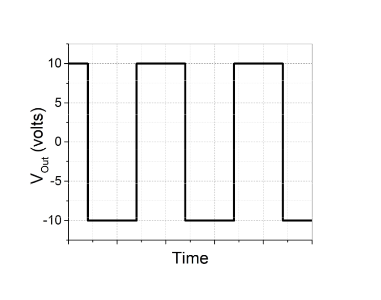
\includegraphics[width=0.8\linewidth]{figs/1.png}
        \label{fig:ann_label}
    \end{figure}
    
  \item[(B)]
  \setcounter{figure}{1}
    \begin{figure}[h]
        \centering
        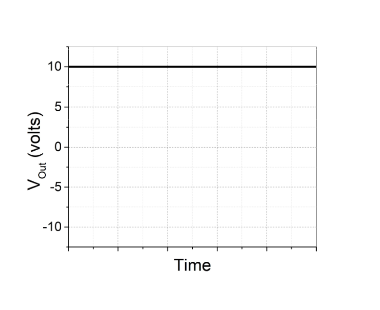
\includegraphics[width=0.8\linewidth]{figs/2.png}
        \label{fig:sww_label}
    \end{figure}
    
  \item[(C)]
  \setcounter{figure}{2}
    \begin{figure}[h]
        \centering
        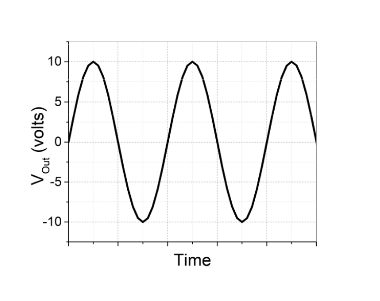
\includegraphics[width=0.8\linewidth]{figs/3.png}
        \label{fig:avv_label}
    \end{figure}
    
  \item[(D)]
  \setcounter{figure}{3}
    \begin{figure}[h]
        \centering
        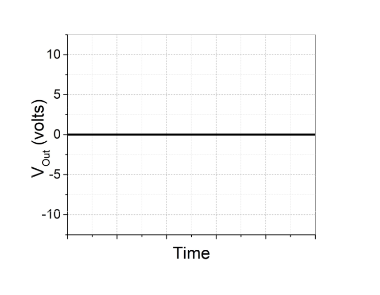
\includegraphics[width=0.8\linewidth]{figs/4.png}
        \label{fig:abb_label}
    \end{figure}
\end{enumerate}

\hfill{(GATE PH 2022)}\\
\textbf{Solution:} \\
Given circuit is a Schmitt Trigger circuit. In this output will be always saturated, i.e., limited between \( +V_{\text{sat}} \) to \( -V_{\text{sat}} \).
So,answer is (A)
\end{document}

